%%% ====================================================================
%%% Início da parte textual do documento.


%%% Configuração do espaçamento entre títulos e texto
\setlength{\afterchapskip}{1.5cm minus \baselineskip}


\chapter{Resultados}
\label{cha:resultados}

Esse capítulo contém os resultados da aplicação e dos estudos de casos aplicados.

\section{Aplicação}

\subsection{Diagrama de Classes}

Com auxílio da ferramenta \textit{Astah Community}, foi desenvolvido o seguinte Diagrama de Classes, apresentado na figura \ref{fig:diagramaClasses}:

\begin{figure}[H]
	\centering
	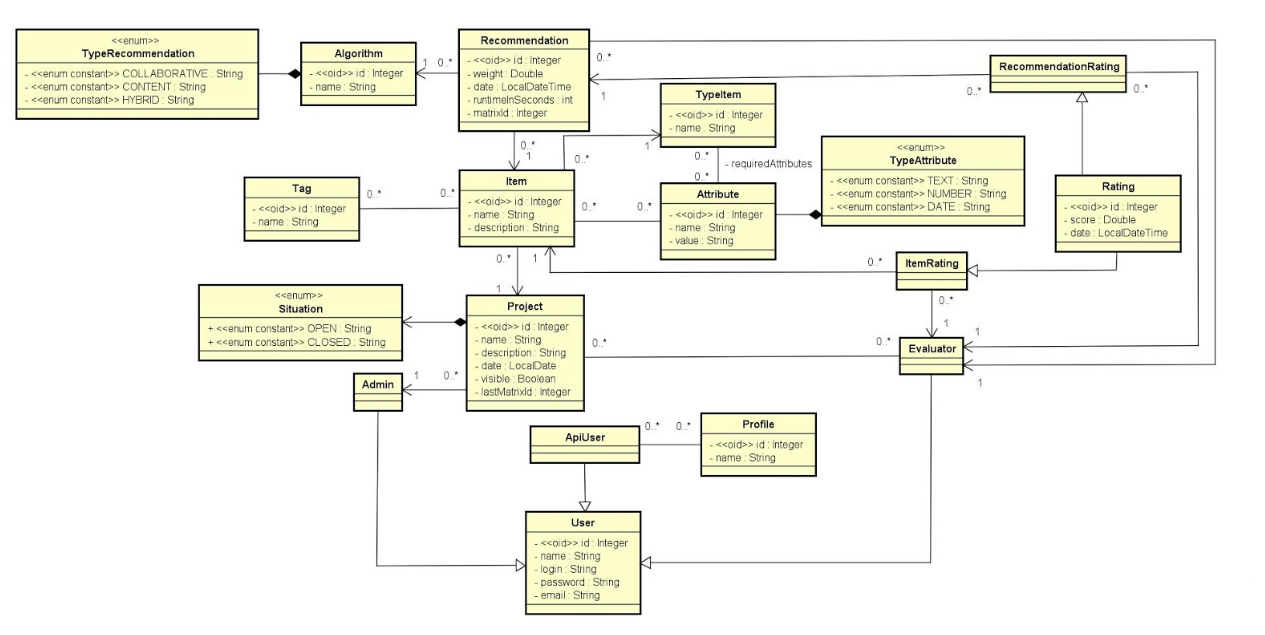
\includegraphics[width=1\linewidth]{imagens/diagramaClasses.PNG}
	\caption[Diagrama de Classes]{Diagrama de Classes}
    \label{fig:diagramaClasses}
\end{figure}

\subsection{API de Recomendação}

Foi desenvolvido uma aplicação backend aberta para uso e modificações. O código fonte de aplicação está disponível no \href{https://github.com/herikLorencao/srh-backend}{GitHub} \footnote{Link do repositório: https://github.com/herikLorencao/srh-backend} podendo ser modificado e adaptado.

Foram desenvolvidos um total de 90 endpoints para a API, que incluem desde cadastros até rotinas de autenticação e recomendação. Todas as rotas estão documentadas e disponíveis no serviço \href{https://documenter.getpostman.com/view/6420672/T1LVA4ST}{Postman} \footnote{Link dos endpoints da API: https://documenter.getpostman.com/view/6420672/T1LVA4ST} para acesso.

\section{Estudo de Caso: Educacional}

\subsection{Contexto}

O intuito deste estudo de caso foi recomendar exercícios aos alunos que pudessem auxiliar significativamente com seu aprendizado no conteúdo estudado.

Para desenvolvendo do estudo de caso, foi selecionada uma turma do curso técnico de Informática Integrado ao Ensino Médio do IFES - Campus Cachoeiro de Itapemirim. O objetivo era o de realizar perguntas relacionadas ao tema de estruturas de controle, na disciplina de Programação I.

Desse modo, o questionário foi aplicado na turma sendo pedido que todos os alunos respondessem todas as perguntas. Para avaliar a assertividade do sistema de recomendação, foram retiradas, de forma aleatória, um conjunto de 0 à 4 respostas de cada aluno, tendo como objetivo criar um ambiente para recomendação onde fosse possível avaliar a taxa de acerto das notas recomendadas.

Na tabela \ref{table:resultadosEstudoCasoEdu} é possível visualizar os dados acerca da pesquisa realizada:

\begin{table}[H]
\centering
\begin{tabular}{|c|c|}
\hline
\textbf{Itens}          & \textbf{Quantidade} \\ \hline
Número de alunos        & 29                  \\ \hline
Número de perguntas     & 9                   \\ \hline
Número de avaliações    & 214                 \\ \hline
Número de tags          & 9                   \\ \hline
Número de recomendações & 47                  \\ \hline
\end{tabular}
\label{table:resultadosEstudoCasoEdu} 
\end{table}

\subsection{Análise Descritiva}

Utilizando-se da estatística descritiva, pode-se avaliar a porcentagem de recomendações que foram aceitas pelos usuários do sistema, verificando, desse modo, sua taxa de acerto. Na figura \ref{fig:analiseDescritiva}, é possível avaliar os resultados obtidos nas recomendações como também as notas avaliadas pelos alunos para cada pergunta. A partir desses dados é possível realizar o processo de estatística descritiva.

\begin{figure}[H]
	\centering
	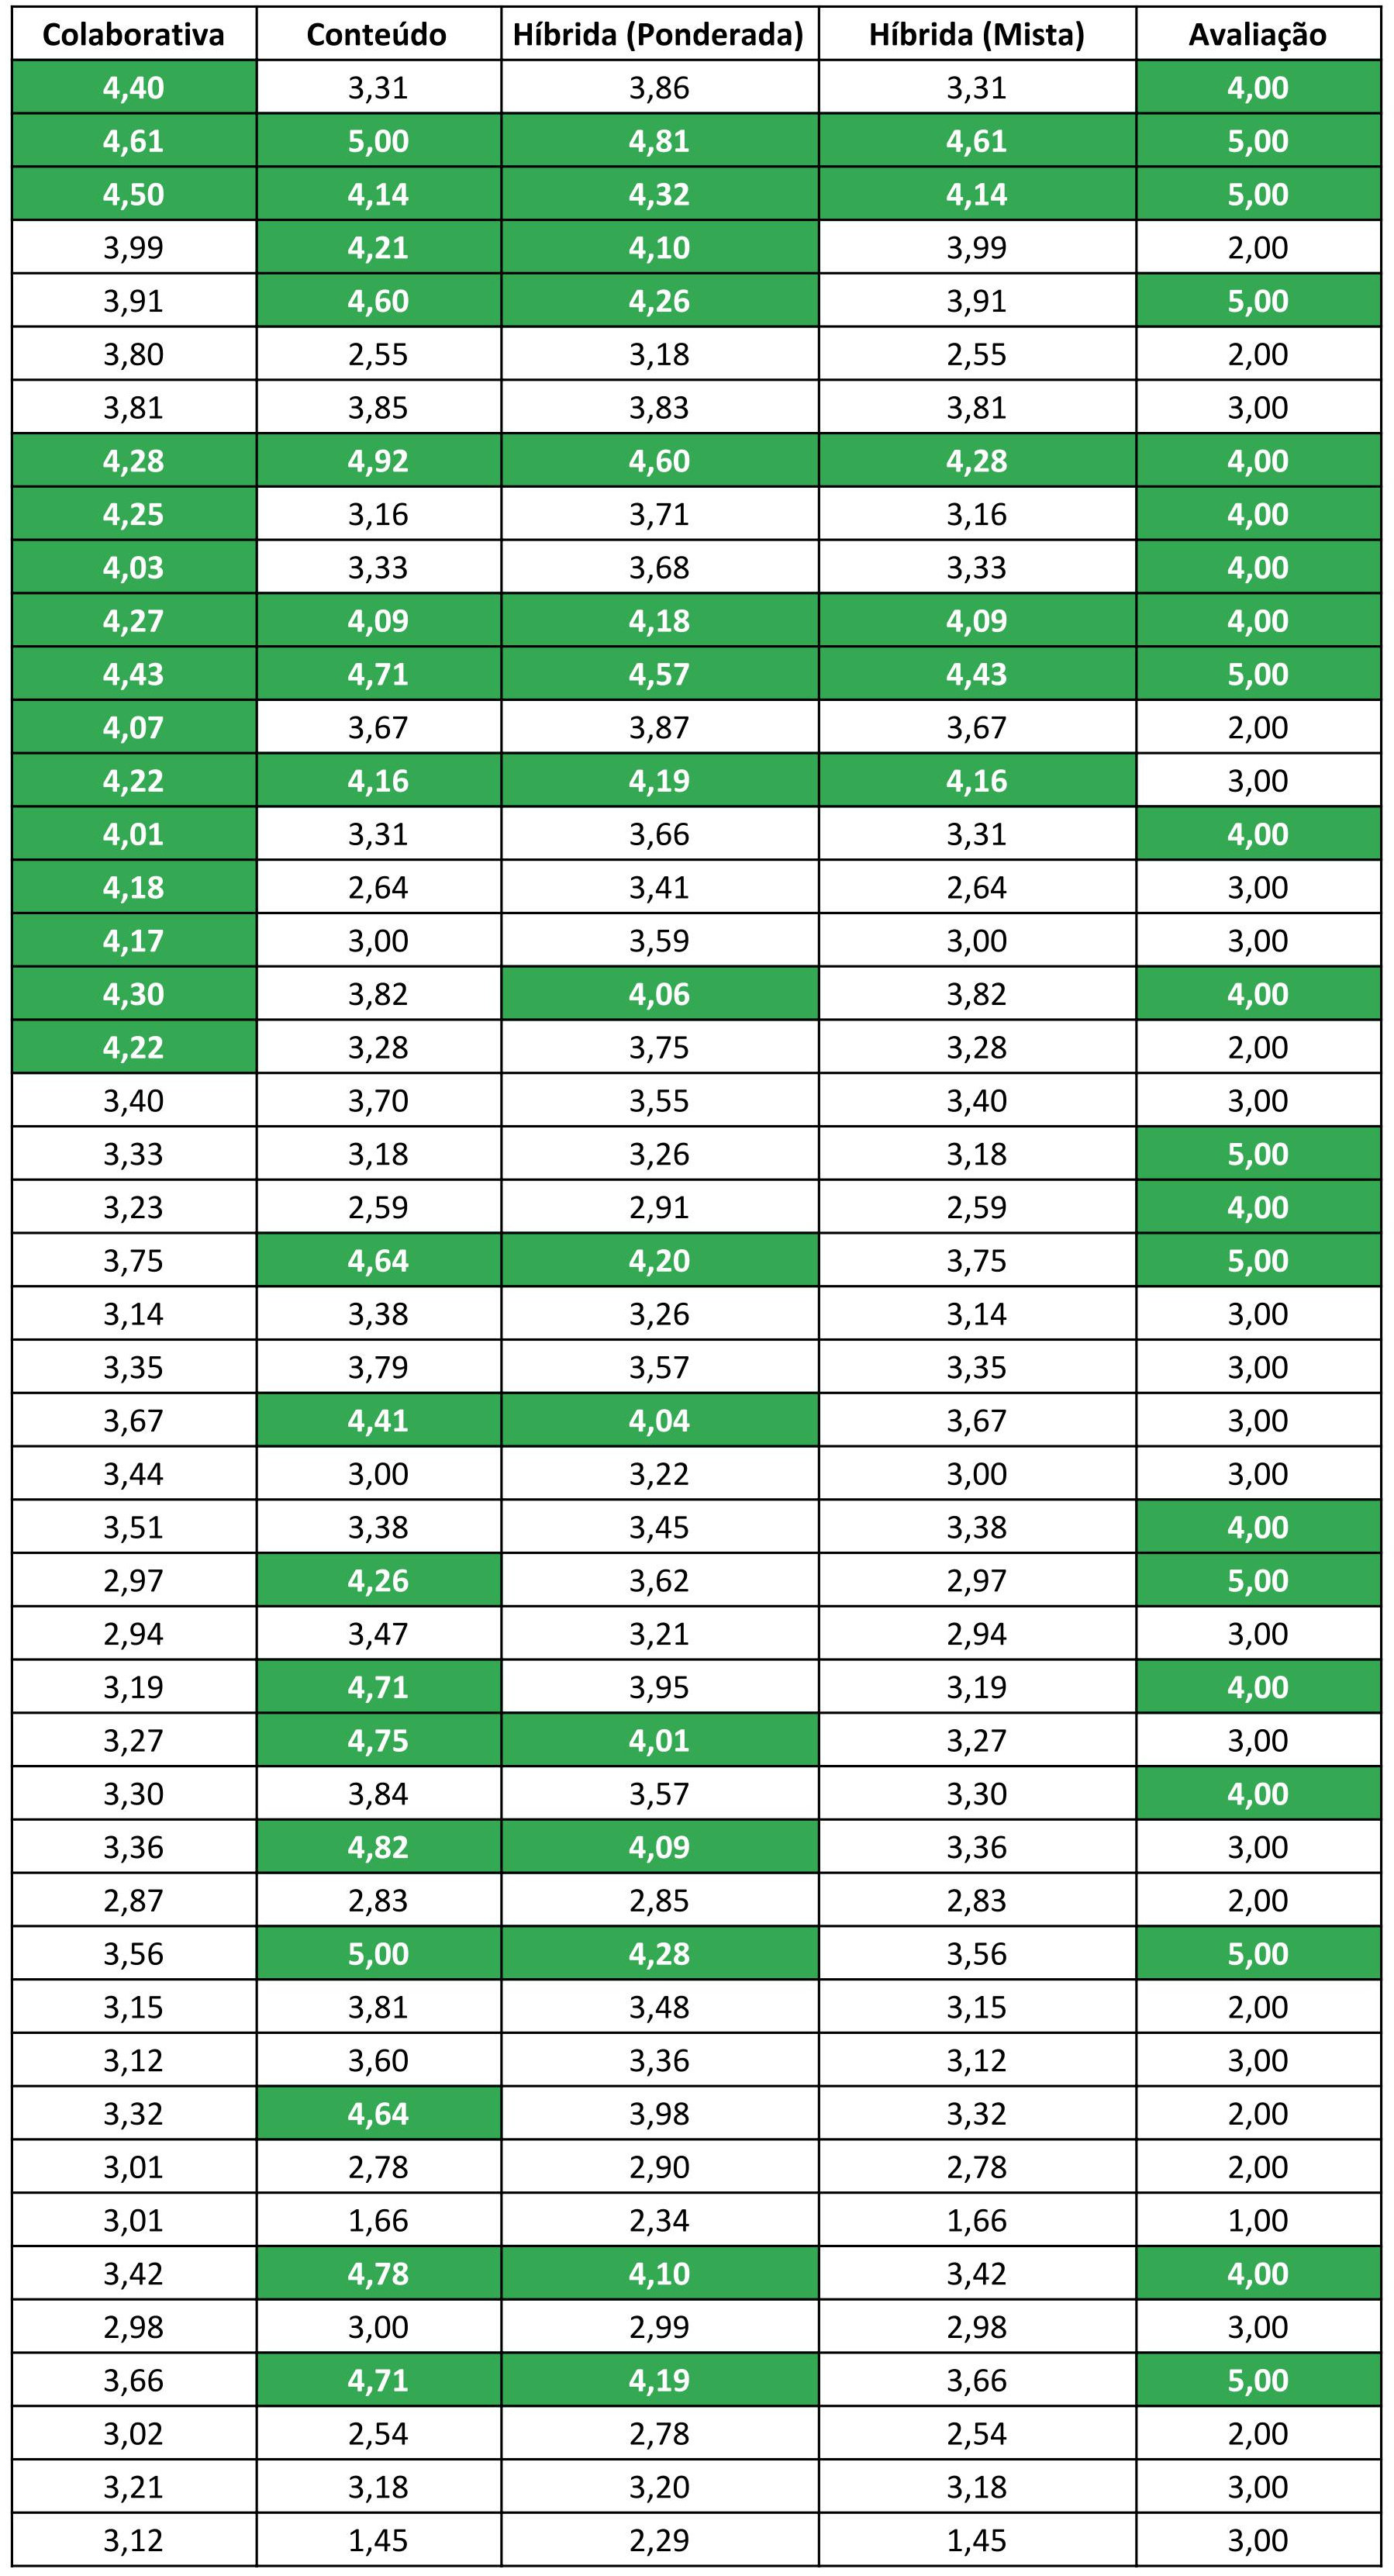
\includegraphics[width=0.8\linewidth]{imagens/estatisticaDescritiva.jpg}
	\caption[Estatística Descritiva]{Estatística Descritiva}
    \label{fig:analiseDescritiva}
\end{figure}

Avaliando as células marcadas na cor verde na figura \ref{fig:analiseDescritiva}, que representam os itens recomendados (notas maiores que o ponto de corte, definido como 4), é possível visualizar a quantidade de acertos e erros das abordagens de recomendação em relação as notas avaliadas pelos usuários. Esses dados são apresentados na figura \ref{fig:analiseDescritivaTaxas}:

\begin{figure}[H]
	\centering
	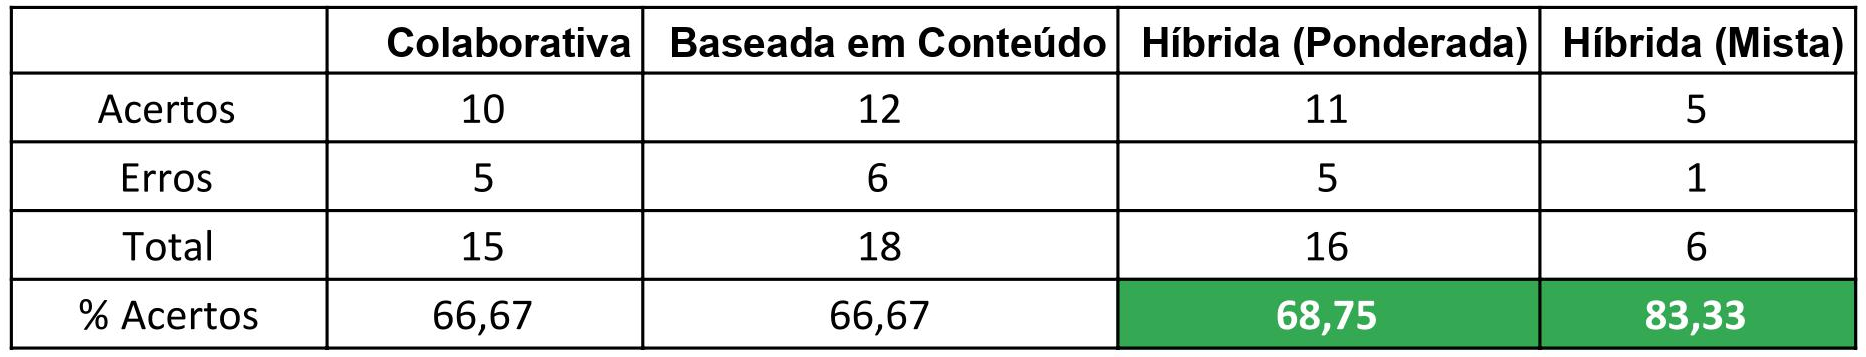
\includegraphics[width=.9\linewidth]{imagens/analiseDescritivaTaxas.jpg}
	\caption[Taxas da Estatística Descritiva]{Taxas da Estatística Descritiva}
    \label{fig:analiseDescritivaTaxas}
\end{figure}

A partir dos dados disponíveis na figura \ref{fig:analiseDescritivaTaxas}, conclui-se que as abordagens híbridas (marcadas com a cor verde) obtiveram um resultado superior as abordagens colaborativas e baseada em conteúdo no estudo analisado. Vale ressaltar o resultado obtido na abordagem híbrida mista, que apresentou um resultado 16,66\% superior as abordagens não híbridas.

\subsection{Testes em T}

Como forma de avaliar os resultados sobre outra perspectiva e metodologia, foram realizados os testes em T que representam outra forma de análise estatística. Nesse tipo de análise, é buscado verificar a diferença entre as médias das recomendações, sendo que quando menor for essa distância melhor o resultado, visto que isso significa que as recomendações estão retornando valores estatisticamente iguais aos avaliados pelos usuários.

\begin{figure}[H]
	\centering
	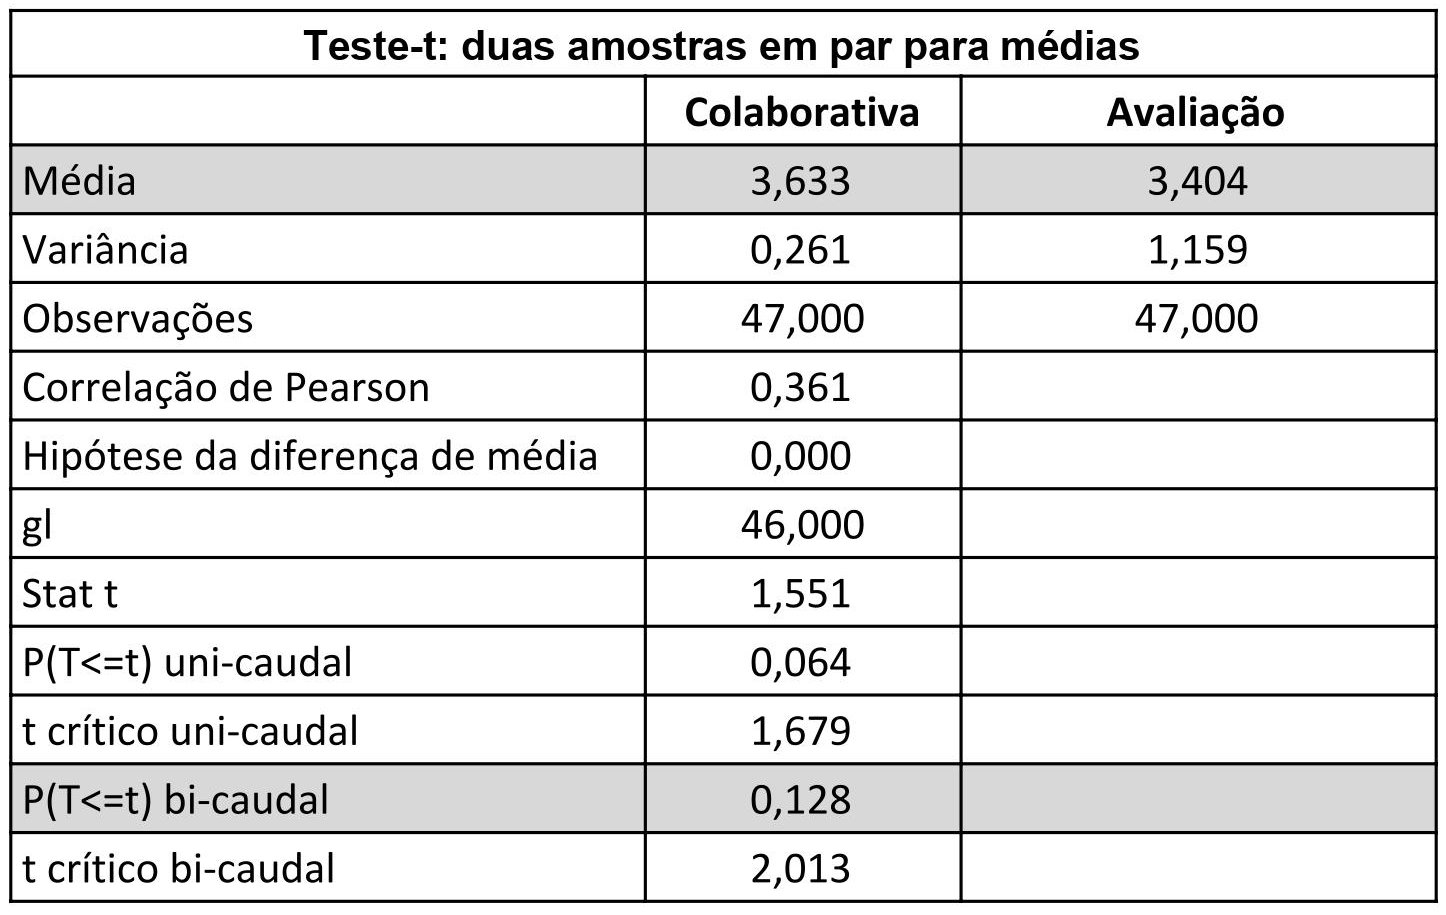
\includegraphics[width=.7\linewidth]{imagens/testeTColaborativa.jpg}
	\caption[Teste T: Filtragem Colaborativa]{Teste T: Filtragem Colaborativa}
    \label{fig:testeTColaborativa}
\end{figure}

A partir dos resultados obtidos na figura \ref{fig:testeTColaborativa}, pode-se observar que o valor de \textbf{P(t<=t) bi-caudal} é superior a \textbf{0,05}. Isso significa que as recomendações para filtragem colaborativa foram boas, uma vez que apresentam similaridade com as avaliações dos usuários.

\begin{figure}[H]
	\centering
	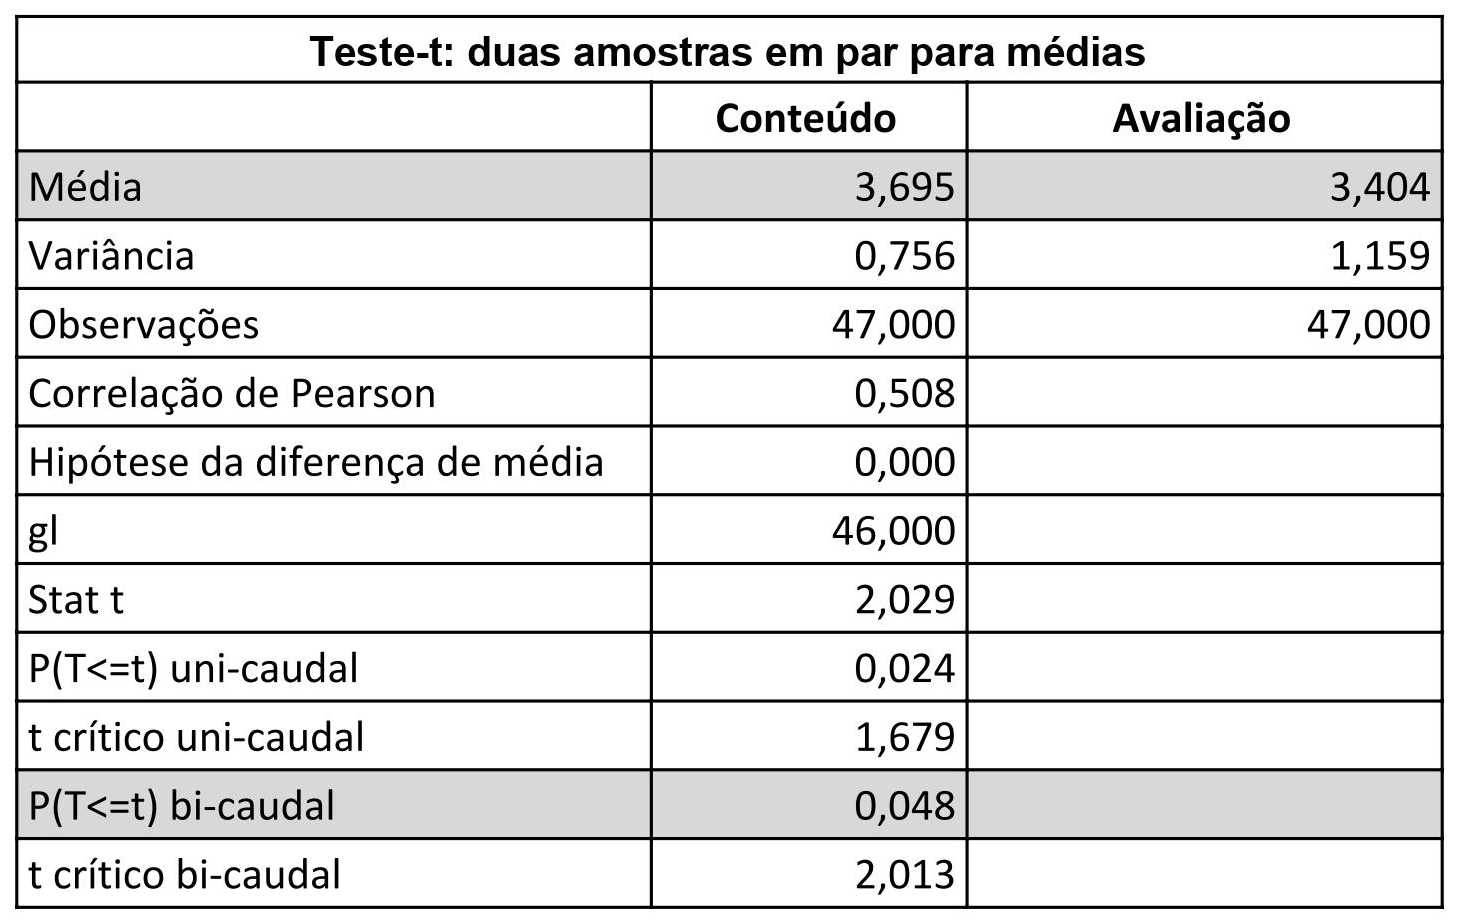
\includegraphics[width=.7\linewidth]{imagens/testeTConteudo.jpg}
	\caption[Teste T: Filtragem Baseada em Conteúdo]{Teste T: Filtragem Baseada em Conteúdo}
    \label{fig:testeTConteudo}
\end{figure}

Os resultados para filtragem baseada em conteúdo, apresentados na figura \ref{fig:testeTConteudo} demonstram um valor para \textbf{P(t<=t) bi-caudal} inferior a \textbf{0,05}. Com isso, é observado que existem uma divergência entre os resultados das recomendações baseadas em conteúdo se comparado com as avaliações dos usuários.

\begin{figure}[H]
	\centering
	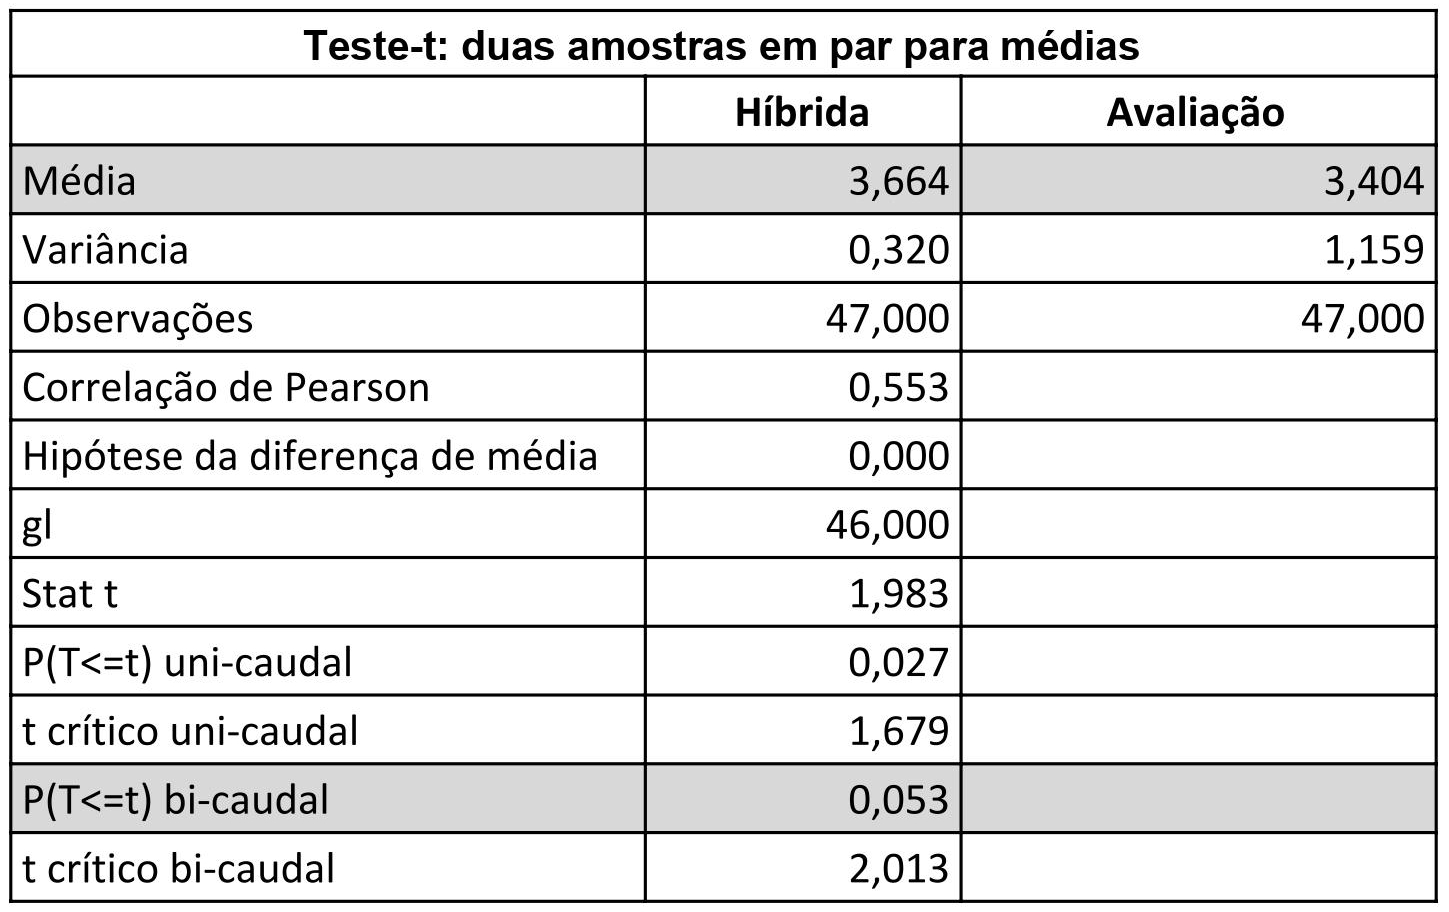
\includegraphics[width=.7\linewidth]{imagens/testeTPonderada.jpg}
	\caption[Teste T: Filtragem Híbrida Ponderada]{Filtragem Híbrida Ponderada}
    \label{fig:testeTPonderado}
\end{figure}

A partir das informações mostradas na figura \ref{fig:testeTPonderado}, é possível analisar que o valor \textbf{P(t<=t) bi-caudal} é superior a \textbf{0,05}. Isso demonstra que as recomendações geradas na filtragem híbrida ponderada apresentam similaridade com as avaliações dos usuários.

\begin{figure}[H]
	\centering
	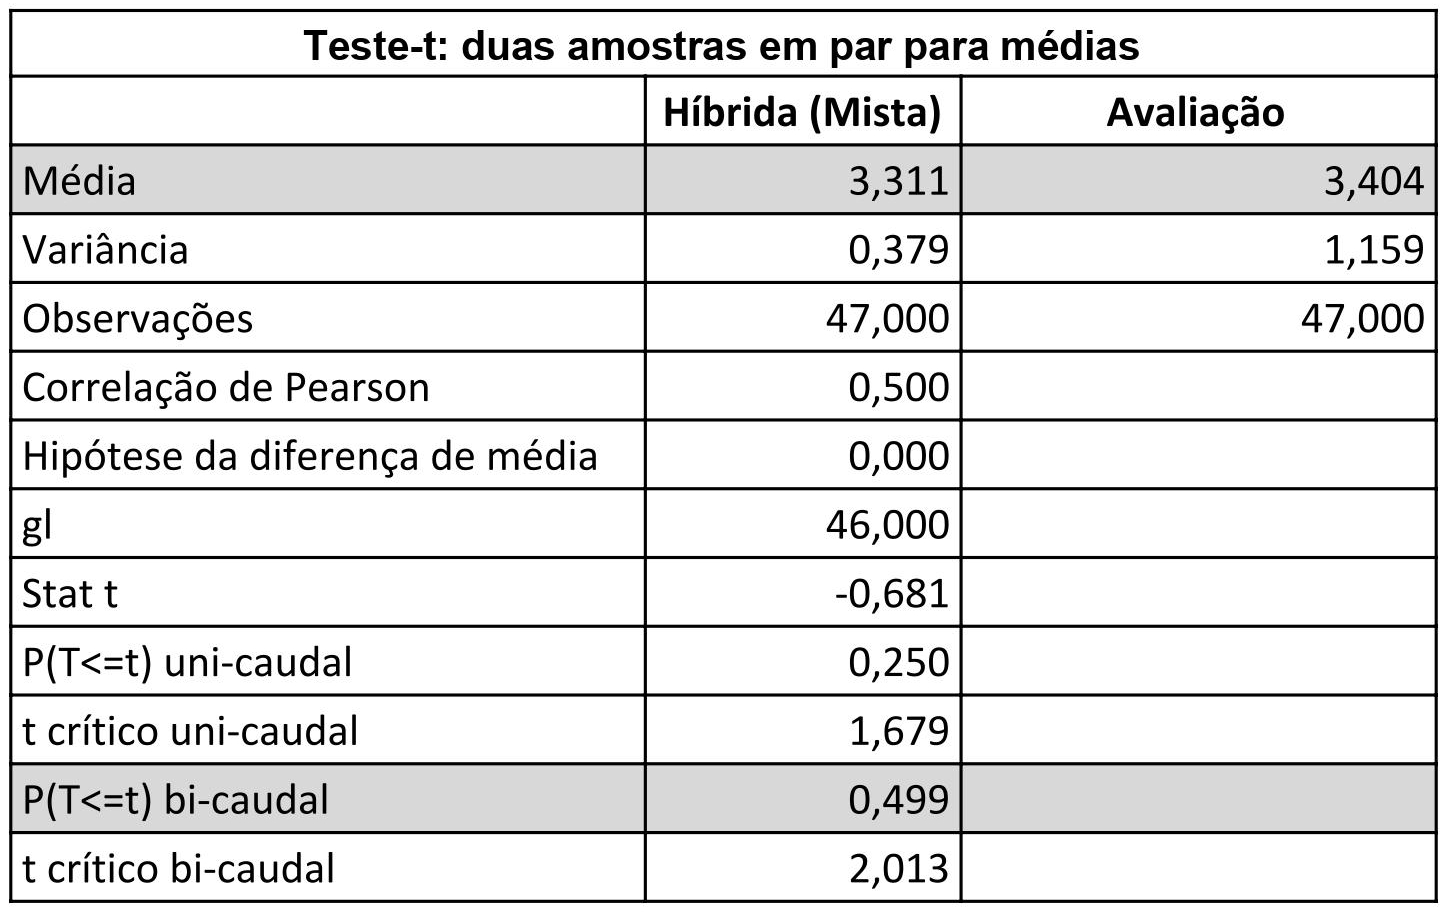
\includegraphics[width=.7\linewidth]{imagens/testeTMisto.jpg}
	\caption[Teste T: Filtragem Híbrida Mista]{Filtragem Híbrida Mista}
    \label{fig:testeTMisto}
\end{figure}

Os resultados da filtragem híbrida mista, apresentados na figura \ref{fig:testeTMisto} demonstram que o valor \textbf{P(t<=t) bi-caudal} é inferior a \textbf{0,05}. Desse modo, é possível observar que existem divergências entre os resultados apresentados pela filtragem híbrida mista e as avaliações dos usuários.